% questions.tex —— 2005 年·普通高等学校招生考试·全国卷Ⅲ·理科 · 题目内容片段（无答案）
% 由 tools/generate_projects.py 依来源总账自 2005/2005_数学真题_全国卷Ⅲ理科_试题.md 生成，勿手改（改源 MD 后重跑）

\begin{question}
\gkti{1}已知 $\alpha$ 为第三象限角，则 $\dfrac{\alpha}{2}$ 所在的象限是\mbox{（　　）}

\begin{gkopts}(2)
\task A．第一或第二象限
\task B．第二或第三象限
\task C．第一或第三象限
\task D．第二或第四象限
\end{gkopts}

\end{question}
\begin{question}
\gkti{2}已知过点 $A(-2, m)$ 和 $B(m, 4)$ 的直线与直线 $2x + y - 1 = 0$ 平行，则 $m$ 的值为\mbox{（　　）}

\begin{gkopts}(4)
\task A．$0$
\task B．$-8$
\task C．$2$
\task D．$10$
\end{gkopts}

\end{question}
\begin{question}
\gkti{3}在 $(x - 1)(x + 1)^8$ 的展开式中 $x^5$ 的系数是\mbox{（　　）}

\begin{gkopts}(4)
\task A．$-14$
\task B．$14$
\task C．$-28$
\task D．$28$
\end{gkopts}

\end{question}
\begin{question}
\gkti{4}设三棱柱 $ABC - A_1B_1C_1$ 的体积为 $V$，$P$、$Q$ 分别是侧棱 $AA_1$、$CC_1$ 上的点，且 $PA = QC_1$，则四棱锥 $B - APQC$ 的体积为\mbox{（　　）}

\begin{gkopts}(4)
\task A．$\dfrac{1}{6}V$
\task B．$\dfrac{1}{4}V$
\task C．$\dfrac{1}{3}V$
\task D．$\dfrac{1}{2}V$
\end{gkopts}

\end{question}
\begin{question}
\gkti{5}$\lim\limits_{x \to 1}\left(\dfrac{1}{x^2 - 3x + 2} - \dfrac{2}{x^2 - 4x + 3}\right) =$\mbox{（　　）}

\begin{gkopts}(4)
\task A．$-\dfrac{1}{2}$
\task B．$\dfrac{1}{2}$
\task C．$-\dfrac{1}{6}$
\task D．$\dfrac{1}{6}$
\end{gkopts}

\end{question}
\begin{question}
\gkti{6}若 $a = \dfrac{\ln 2}{2}$，$b = \dfrac{\ln 3}{3}$，$c = \dfrac{\ln 5}{5}$，则\mbox{（　　）}

\begin{gkopts}(4)
\task A．$a < b < c$
\task B．$c < b < a$
\task C．$c < a < b$
\task D．$b < a < c$
\end{gkopts}

\end{question}
\begin{question}
\gkti{7}设 $0 \leqslant x \leqslant 2\pi$，且 $\sqrt{1 - \sin 2x} = \sin x - \cos x$，则\mbox{（　　）}

\begin{gkopts}(1)
\task A．$0 \leqslant x \leqslant \pi$
\task B．$\dfrac{\pi}{4} \leqslant x \leqslant \dfrac{7\pi}{4}$
\task C．$\dfrac{\pi}{4} \leqslant x \leqslant \dfrac{5\pi}{4}$
\task D．$\dfrac{\pi}{2} \leqslant x \leqslant \dfrac{3\pi}{2}$
\end{gkopts}

\end{question}
\begin{question}
\gkti{8}$\dfrac{2\sin 2\alpha}{1 + \cos 2\alpha} \cdot \dfrac{\cos^2 \alpha}{\cos 2\alpha} =$\mbox{（　　）}

\begin{gkopts}(4)
\task A．$\tan \alpha$
\task B．$\tan 2\alpha$
\task C．$1$
\task D．$\dfrac{1}{2}$
\end{gkopts}

\end{question}
\begin{question}
\gkti{9}已知双曲线 $x^2 - \dfrac{y^2}{2} = 1$ 的焦点为 $F_1$、$F_2$，点 $M$ 在双曲线上且 $\overrightarrow{MF_1} \cdot \overrightarrow{MF_2} = 0$，则点 $M$ 到 $x$ 轴的距离为\mbox{（　　）}

\begin{gkopts}(2)
\task A．$\dfrac{4}{3}$
\task B．$\dfrac{5}{3}$
\task C．$\dfrac{2\sqrt{3}}{3}$
\task D．$\sqrt{3}$
\end{gkopts}

\end{question}
\begin{question}
\gkti{10}设椭圆的两个焦点分别为 $F_1$、$F_2$，过 $F_2$ 作椭圆长轴的垂线交椭圆于点 $P$，若 $\triangle F_1PF_2$ 为等腰直角三角形，则椭圆的离心率是\mbox{（　　）}

\begin{gkopts}(2)
\task A．$\dfrac{\sqrt{2}}{2}$
\task B．$\dfrac{\sqrt{2} - 1}{2}$
\task C．$2 - \sqrt{2}$
\task D．$\sqrt{2} - 1$
\end{gkopts}

\end{question}
\begin{question}
\gkti{11}不共面的四个定点到平面 $\alpha$ 的距离都相等，这样的平面 $\alpha$ 共有\mbox{（　　）}

\begin{gkopts}(4)
\task A．$3$ 个
\task B．$4$ 个
\task C．$6$ 个
\task D．$7$ 个
\end{gkopts}

\end{question}
\begin{question}
\gkti{12}计算机中常用十六进制是逢 $16$ 进 $1$ 的计数制，采用数字 $0 \sim 9$ 和字母 $A \sim F$ 共 $16$ 个计数符号，这些符号与十进制的数的对应关系如下表：

\begin{center}
\begingroup\setlength{\tabcolsep}{4pt}
\begin{tabular}{lcccccccc}
\toprule
十六进制 & 0 & 1 & 2 & 3 & 4 & 5 & 6 & 7 \\
\midrule
十进制 & 0 & 1 & 2 & 3 & 4 & 5 & 6 & 7 \\
十六进制 & 8 & 9 & A & B & C & D & E & F \\
十进制 & 8 & 9 & 10 & 11 & 12 & 13 & 14 & 15 \\
\bottomrule
\end{tabular}
\endgroup
\end{center}

例如，用十六进制表示：$E + D = 1B$，则 $A \times B =$\mbox{（　　）}

\begin{gkopts}(4)
\task A．$6E$
\task B．$72$
\task C．$5F$
\task D．$B0$
\end{gkopts}

\end{question}
\begin{question}
\gkti{13}已知复数 $z_0 = 3 + 2\mathrm{i}$，复数 $z$ 满足 $z \cdot z_0 = 3z + z_0$，则复数 $z =$＿＿＿＿＿＿．

\end{question}
\begin{question}
\gkti{14}已知向量 $\overrightarrow{OA} = (k, 12)$，$\overrightarrow{OB} = (4, 5)$，$\overrightarrow{OC} = (-k, 10)$，且 $A$、$B$、$C$ 三点共线，则 $k =$＿＿＿＿＿＿．

\end{question}
\begin{question}
\gkti{15}设 $l$ 为平面上过点 $(0, 1)$ 的直线，$l$ 的斜率等可能地取 $-2\sqrt{2}$、$-\sqrt{3}$、$-\dfrac{\sqrt{5}}{2}$、$0$、$\dfrac{\sqrt{5}}{2}$、$\sqrt{3}$、$2\sqrt{2}$，用 $\xi$ 表示坐标原点到 $l$ 的距离，则随机变量 $\xi$ 的数学期望 $E\xi =$＿＿＿＿＿＿．

\end{question}
\begin{question}
\gkti{16}已知在 $\triangle ABC$ 中，$\angle ACB = 90^\circ$，$BC = 3$，$AC = 4$，$P$ 是 $AB$ 上的点，则点 $P$ 到 $AC$、$BC$ 的距离乘积的最大值是＿＿＿＿＿＿．

\end{question}
\begin{question}
\gkti{17}设甲、乙、丙三台机器是否需要照顾相互之间没有影响．已知在某一小时内，甲、乙都需要照顾的概率为 $0.05$，甲、丙都需要照顾的概率为 $0.1$，乙、丙都需要照顾的概率为 $0.125$．

(1) 求甲、乙、丙每台机器在这个小时内需要照顾的概率分别是多少；

(2) 计算这个小时内至少有一台需要照顾的概率．

\Needspace{0.4\textheight}
\end{question}
\begin{question}
\gkti{18}如图，在四棱锥 $V - ABCD$ 中，底面 $ABCD$ 是正方形，侧面 $VAD$ 是正三角形，平面 $VAD \perp$ 底面 $ABCD$．

(1) 证明：$AB \perp$ 平面 $VAD$；

(2) 求面 $VAD$ 与面 $VDB$ 所成的二面角的大小．
\nopagebreak[4]
\begin{center}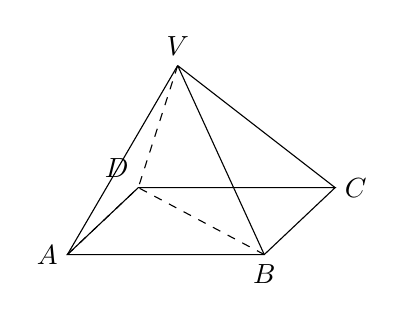
\begin{tikzpicture}[scale=1.0]
  \coordinate (V) at (0.1,2.4);
  \coordinate (A) at (-1.3,0);
  \coordinate (B) at (1.2,0);
  \coordinate (C) at (2.1,0.85);
  \coordinate (D) at (-0.4,0.85);
  \draw (V) -- (A) (V) -- (B) (V) -- (C);
  \draw (A) -- (B) -- (C) -- (D) -- cycle;
  \draw[dashed] (V) -- (D);
  \draw[dashed] (A) -- (D);
  \draw[dashed] (B) -- (D);
  \node[above] at (V) {$V$};
  \node[left] at (A) {$A$};
  \node[below] at (B) {$B$};
  \node[right] at (C) {$C$};
  \node[above left] at (D) {$D$};
\end{tikzpicture}
\end{center}
\nopagebreak[4]
\end{question}
\begin{question}
\gkti{19}$\triangle ABC$ 中，内角 $A$、$B$、$C$ 的对边分别为 $a$、$b$、$c$，已知 $a$、$b$、$c$ 成等比数列，$\cos B = \dfrac{3}{4}$．

(1) 求 $\cot A + \cot C$ 的值；

(2) 设 $\overrightarrow{BA} \cdot \overrightarrow{BC} = \dfrac{3}{2}$，求 $a + c$ 的值．

\end{question}
\begin{question}
\gkti{20}在等差数列 $\{a_n\}$ 中，公差 $d \neq 0$，$a_2$ 是 $a_1$ 与 $a_4$ 的等比中项．已知数列 $a_1, a_3, a_{k_1}, a_{k_2}, \cdots, a_{k_n}, \cdots$ 成等比数列，求数列 $\{k_n\}$ 的通项 $k_n$．

\end{question}
\begin{question}
\gkti{21}设 $A(x_1, y_1)$，$B(x_2, y_2)$ 两点在抛物线 $y = 2x^2$ 上，$l$ 是 $AB$ 的垂直平分线．

(1) 当且仅当 $x_1 + x_2$ 取何值时，直线 $l$ 经过抛物线的焦点 $F$？证明你的结论；

(2) 当直线 $l$ 的斜率为 $2$ 时，求 $l$ 在 $y$ 轴上截距的取值范围．

\end{question}
\begin{question}
\gkti{22}已知函数 $f(x) = \dfrac{4x^2 - 7}{2 - x}$，$x \in [0, 1]$．

(1) 求 $f(x)$ 的单调区间和值域；

(2) 设 $a \geqslant 1$，函数 $g(x) = x^3 - 3a^2x - 2a$，$x \in [0, 1]$．若对于任意 $x_1 \in [0, 1]$，总存在 $x_0 \in [0, 1]$，使得 $g(x_0) = f(x_1)$ 成立，求 $a$ 的取值范围．

\end{question}